\chapter{一致性}

\section{原理}

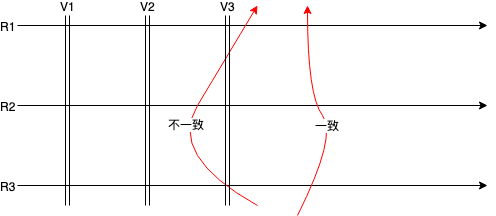
\includegraphics[width=11cm]{../imgs/consistency-splice.png}

从逻辑上讲,一致性是由任一对象的变更历史决定的。强一致性要求:
\begin{enumbox}
\item 任一对象的多个副本/分片,可以看作有限状态机,须按同一顺序执行变更。变更通常包括写IO和内部修复IO。
\item 已提交的写不能丢失
\item 能读到最新数据
\end{enumbox}

相比于副本机制,EC的各分片具有严格顺序。

从实现机制上来看,副本或EC的一致性,需要从\hl{对象版本、控制器和日志}几个方面来考虑。

恢复过程的关键是\hl{选择到正确的副本/分片}。分为几种情况:
\begin{enumbox}
\item EC的节点故障
\item EC的磁盘故障
\item 副本
\end{enumbox}

\section{副本一致性}

现象:观察到恢复完成后,有时vdi对象并不一致。

\todo{副本一致性}目前副本的一致性实现,机制上恐有问题。
恢复的选择步骤,各个副本独立运行选择过程,所依据的并非该对象各个副本的全局信息,而是相当局部的信息。
并不能保证一定选择到正确副本。

需要参考EC一致性的机制,选出primary协调IO和recovery活动。
副本的选择步骤相对简单:可用的最大版本的副本,以之为权威副本,覆盖其余。

\section{EC一致性}

\subsection{对象版本}

从概念上来说,SSAN按epoch组织对象,节点故障时提升epoch,磁盘故障时epoch不变,
通过强制升级epoch来模拟节点/磁盘混合故障。

epoch是集群级别的版本,epoch内节点成员关系不变。在SSAN实现里epoch被用作粗粒度的对象版本。

\subsection{控制器}

IO控制器是gateway,SSAN原始实现无恢复控制器,后针对任一对象引入primary数据分片作为恢复控制器。
这样就形成\hl{IO和恢复的双控架构},为了对象一致性,需要同步IO控制器和恢复控制器。

\subsection{日志}

无日志,难以处理特定情况下的恢复问题。比如4+2时,如果成功写入3个数据分片,则过程无法重入,无法
从该不一致状态修复到一致性状态。\hl{对条带对齐的IO,可采用REDO日志replay这个过程}。
维护UNDO日志则相对复杂。

\subsection{对象组织及其cache}
\label{subsec:object-dir}

因为可能在工作目录创建不同epoch的对象,工作目录下的对象名字也要包括epoch。

进一步可以考虑按epoch组织目录,这样可以简化关键操作,比如消除rename和link操作。
磁盘故障时,因为不升级epoch,所以需要特别处理,\hl{校正对象的磁盘位置,但不需要link了}。
需要保证过程的原子性。

维护磁盘对象结构的内存cache,在其上面提供API,合并stale cache和object list cache。
需要实现的API包括:
\begin{enumbox}
\item get\_obj\_list,获取一节点上所有对象的oid
\item get\_obj\_history,获取一个object的历史版本
\item get\_obj\_history2,获取一个object的历史版本,wd==0
\item stale\_cache\_compact,清除无效磁盘相关的记录
\end{enumbox}

\subsection{恢复实例}

恢复实例可以看作有限状态机。在恢复期间,SSAN进程运行一个恢复实例。
如果有新的故障,则执行上下文切换,切换到下一恢复实例。需要保证切换恢复实例过程的正确性。
任一时刻,最多有一个恢复实例在运行。

恢复状态机的每步转换都要满足safety和liveness条件,特别需要注意的是:
\begin{enumbox}
\item update epoch过程务必成功执行
\item 若一节点收不到recover peer,无法进入NOTIFY STANDBY DONE状态
\end{enumbox}

\subsection{TODO}

\begin{enumbox}
\item prepare object list,接收到非法oid
\item do\_event\_loop里ei->name出现乱码
\end{enumbox}

\section{EC一致性的改进之处}

具体见git仓库的提交日志。

\subsection{增强系统可追踪性}

主要通过日志机制来实现。把每个对象、io、恢复实例等等实体看作对象,追踪其生命周期行为,便于分析异常现象。

引入GOTO、SD\_ASSERT macro。

引入COREDUMP

引入RAMDISK

\subsection{create and write采用sync模式}

出现虽然写成功,后来发现对象内容为全零的情况。

\subsection{优化oidlist的索引}

优先修复vdi object。

采用bitmap检索data object和ledger object。\todo{摘除优先修复对象}\hl{数据量大时,优先修复的oid依然效率低}。

\subsection{改进对象组织方式}

参考小节~\ref{subsec:object-dir}

\subsection{改进stale object cache}

改进stale object cache模块,用于追踪对象在磁盘上的分布,可以理解为磁盘目录结构的cache。
通过支持所需API,来替代原来的object list cache和stale cache。同时也方便stale object的GC过程。

\subsection{恢复状态机引入新状态}

重构恢复实例的状态机。

引入RW\_INIT:为了实现没有进入prepare状态的恢复实例,可以切换到下一实例。一旦进入prepare阶段,则切换过程有所不同。
\hl{通用原则是确保rinfo上下文信息的安全性}。在有引用计数的情况下,不能被free掉。

引入RW\_UPDATE\_EPOCH:因为update epoch执行时间过长,为了不堵塞main线程,须放到工作线程中去做。

引入RW\_NOTIFY\_STANDBY\_DONE:放入同步点,以确保object list cache准备妥当,才能保证后续prepare object list过程无误。

避免prepare object list重复入队,导致修复崩溃

\subsection{磁盘空间不足时的恢复过程}

\todo{磁盘空间不足时的恢复过程}可以在finish object list过程,加入检查逻辑。检查项:
\begin{enumbox}
\item 每个disk的容量是否够用(执行hash运算后分布到该磁盘上的对象)
\item 对象的历史版本可能没及时回收
\item 在恢复过程中会有新的create and write
\end{enumbox}

如果不能通过检查,则标记节点状态为NODE\_NOSPC,影响到的操作:
\begin{enumbox}
\item 读写io
\item 退出恢复过程
\end{enumbox}

在此状态下,运行执行删除卷操作,以回收空间。回收完成后,重新进入修复状态。

\subsection{retry机制}

retry机制的使用需要具体分析,内部过程慎用retry,避免堵塞main线程,使系统失去响应能力。

重试次数和timeout值的选择也影响到故障切换时长和IO中断时长。

\subsection{Too many open files}

文件句柄数量控制,由最大1024改为1048576。直接在SSAN进程内设定。

\subsection{scli cluster check的OOM现象}

因为check过程相对低效,导致等待check的队列大量积压,消耗大量内存,引起OOM。
故引入QoS机制,限制队列长度,减少内存消耗。

\subsection{日志缓冲区设定过小,导致日志丢失}

\section{小结}

指导原则
\begin{enumbox}
\item 一致性问题要对标相关参考模型
\item 采用流体动力学模型分析性能瓶颈
\item 工欲善其事必先利其器
\end{enumbox}

工具方面
\begin{enumbox}
\item 完整日志追踪系统,细粒度地追踪程序运行时行为
\item 加入PROFILE日志,辅助分析各个过程的性能特征
\item 多用断言,以捕获程序中的不变式,尽早暴露问题
\item 生成COREDUMP
\item 采用valgrind分析内存问题
\item 采用egrep分析日志,保留相关日志的相对顺序
\item 采用fio的verify和scli cluster check机制验证一致性
\item ***
\item 尽量保障开发和测试环境
\end{enumbox}

egrep的使用示例:
\begin{lstlisting}[language=bash,frame=single]
egrep 'start_recovery|free_recovery_info' ssan.log
egrep 'start_recovery|iops' ssan.log
\end{lstlisting}

关于日志子系统,需要从内容和形式上进一步规范化。
\begin{enumbox}
\item 可动态调整日志等级
\item 管理对象的生命周期活动
\item 捕获尽可能多的上下文信息
\item 提高日志的信息密度
\item 关键字
\end{enumbox}

性能分析
\begin{enumbox}
\item 流出等于流入
\item 下游处理能力大于流入流量
\item 调度能力大于下游处理能力
\end{enumbox}

重点是提升下游节点的处理能力和中间节点的调度能力。
以修复为例,下游处理能力对应恢复性能,调度能力对应main线程的调度能力。

\section{suazku一致性方案}

epoch down set

GFM

\subsection{一致性的判断条件}

clock全等(skip dirty==1)。如果不等,则选取最大的,覆盖其余。

\subsection{IO流程}

\mygraphics{../imgs/rangectl/rep-sessid.png}

\mygraphics{../imgs/rangectl/io-token.png}

降级模式,只有降级模式下才需要序列化clock?

\subsection{恢复过程}

恢复是独立于core线程的外部线程,卷怎么映射到各个恢复线程上?

open并scan卷。

\subsection{故障检测机制}

查询rangectl以确定是否需要恢复?
